% =============================================================================
%  STANDALONE HAF-STD NET ARCHITECTURE DIAGRAM (Clean Version)
%  Compile with: pdflatex hafstd_figure.tex
% =============================================================================
\documentclass[border=12pt]{standalone}

\usepackage{tikz}
\usepackage{amsmath, amssymb}
\usepackage{times}
\usetikzlibrary{shapes, arrows.meta, positioning, calc, fit, backgrounds}

\begin{document}

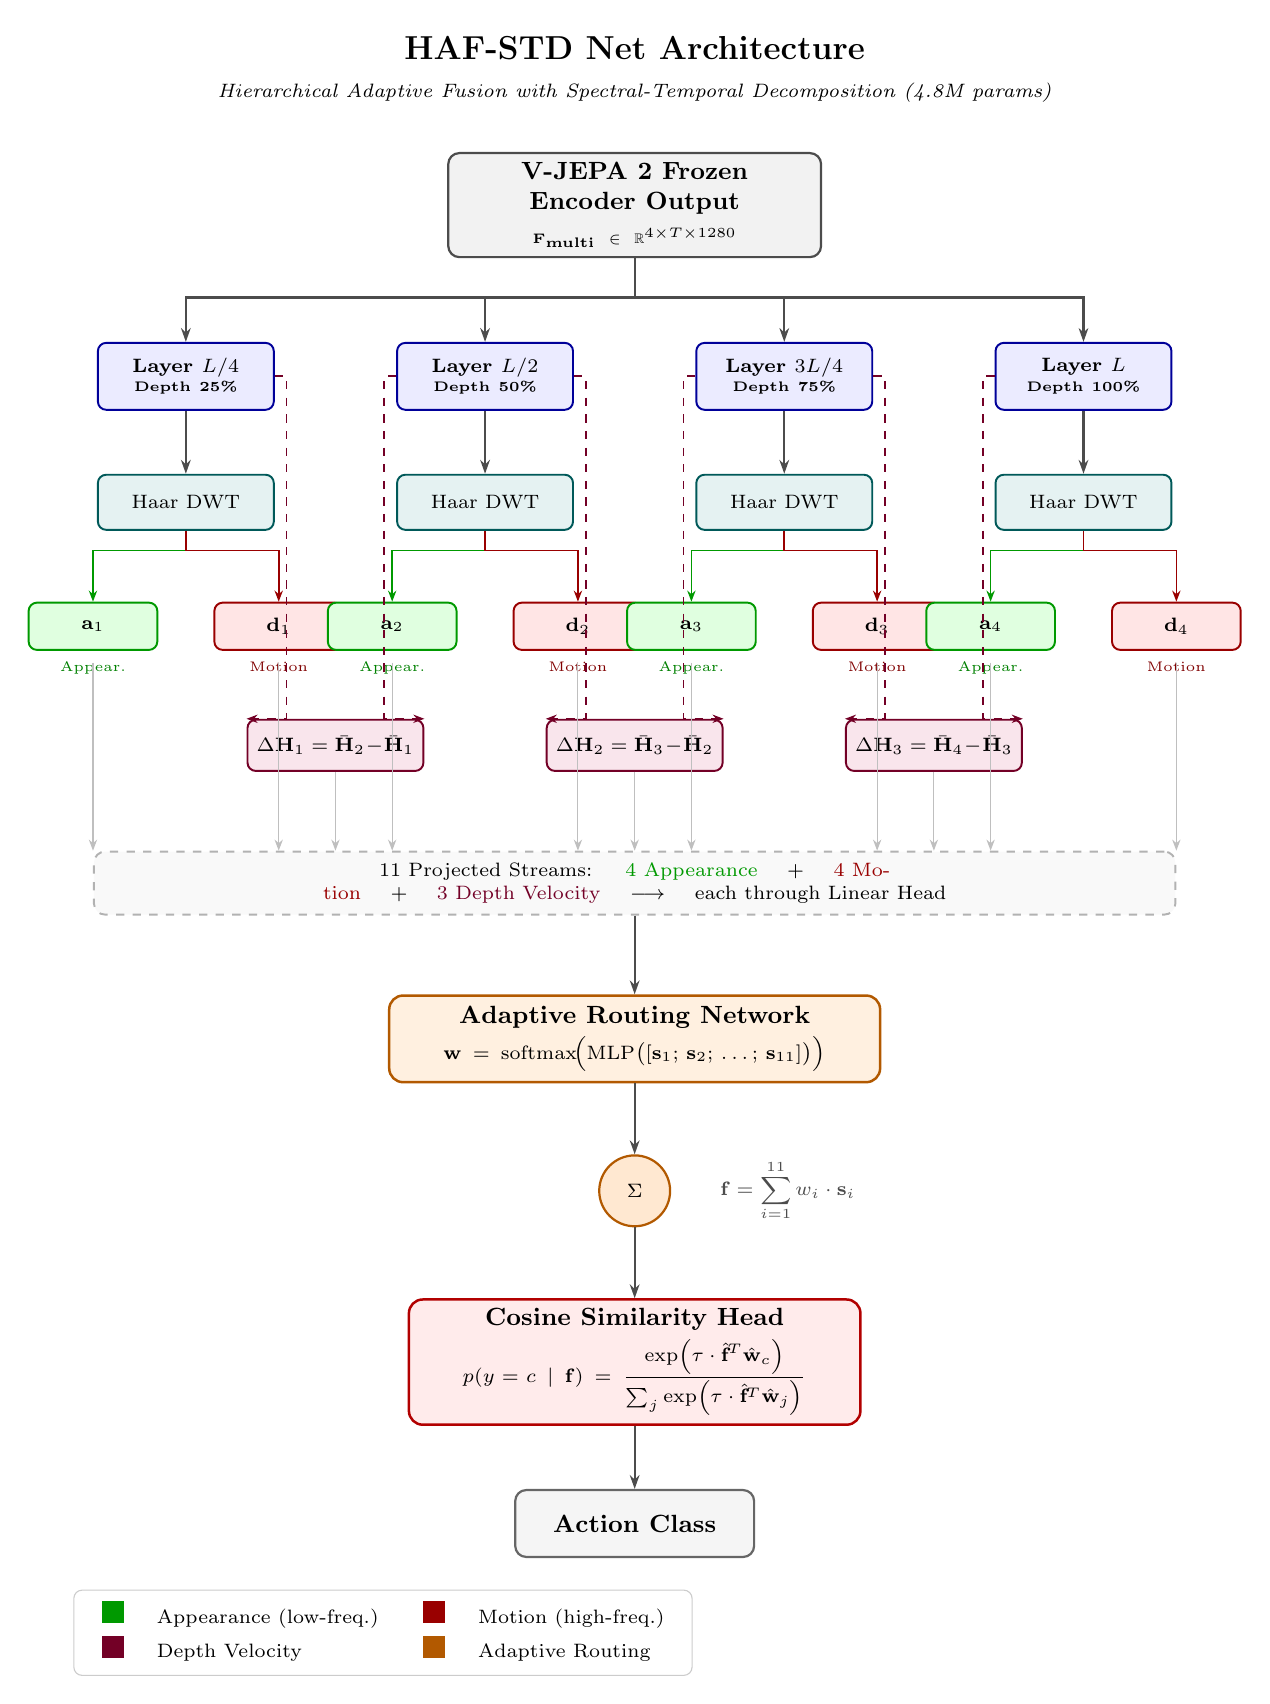
\begin{tikzpicture}[
    % === Node styles ===
    input/.style={rectangle, draw=black!70, fill=gray!10, text width=4.5cm,
        text centered, rounded corners=4pt, minimum height=1.1cm,
        font=\small\bfseries, line width=0.8pt},
    layer/.style={rectangle, draw=blue!60!black, fill=blue!8, text width=2.0cm,
        text centered, rounded corners=3pt, minimum height=0.85cm,
        font=\scriptsize\bfseries, line width=0.7pt},
    dwt/.style={rectangle, draw=teal!70!black, fill=teal!10, text width=2.0cm,
        text centered, rounded corners=3pt, minimum height=0.7cm,
        font=\scriptsize, line width=0.7pt},
    appear/.style={rectangle, draw=green!60!black, fill=green!12, text width=1.4cm,
        text centered, rounded corners=3pt, minimum height=0.6cm,
        font=\scriptsize, line width=0.7pt},
    motion/.style={rectangle, draw=red!60!black, fill=red!10, text width=1.4cm,
        text centered, rounded corners=3pt, minimum height=0.6cm,
        font=\scriptsize, line width=0.7pt},
    velocity/.style={rectangle, draw=purple!60!black, fill=purple!10, text width=2.0cm,
        text centered, rounded corners=3pt, minimum height=0.65cm,
        font=\scriptsize, line width=0.7pt},
    collect/.style={rectangle, draw=gray!60, fill=gray!5, text width=13.5cm,
        text centered, rounded corners=4pt, minimum height=0.8cm,
        font=\scriptsize, line width=0.7pt, dashed},
    router/.style={rectangle, draw=orange!70!black, fill=orange!12, text width=6.0cm,
        text centered, rounded corners=5pt, minimum height=1.1cm,
        font=\small\bfseries, line width=0.9pt},
    fuse/.style={circle, draw=orange!70!black, fill=orange!18, minimum size=0.9cm,
        font=\scriptsize\bfseries, line width=0.8pt},
    classifier/.style={rectangle, draw=red!70!black, fill=red!8, text width=5.5cm,
        text centered, rounded corners=5pt, minimum height=1.1cm,
        font=\small\bfseries, line width=0.9pt},
    outputbox/.style={rectangle, draw=black!60, fill=gray!8, text width=2.8cm,
        text centered, rounded corners=4pt, minimum height=0.85cm,
        font=\small\bfseries, line width=0.8pt},
    arrow/.style={-{Stealth[length=5pt, width=3.5pt]}, thick, color=black!70},
    garrow/.style={-{Stealth[length=4pt, width=3pt]}, semithick, color=green!60!black},
    rarrow/.style={-{Stealth[length=4pt, width=3pt]}, semithick, color=red!60!black},
    parrow/.style={-{Stealth[length=4pt, width=3pt]}, semithick, dashed, color=purple!60!black},
    streamarrow/.style={-{Stealth[length=4pt, width=3pt]}, thin, color=gray!50},
]

% =============================================
% ROW 0: TITLE
% =============================================
\node[font=\large\bfseries] (title) at (0, 0) {HAF-STD Net Architecture};
\node[font=\scriptsize\itshape, below=0.05cm of title] (subtitle)
    {Hierarchical Adaptive Fusion with Spectral-Temporal Decomposition (4.8M params)};

% =============================================
% ROW 1: INPUT
% =============================================
\node[input, below=0.5cm of subtitle] (input)
    {V-JEPA 2 Frozen Encoder Output\\[1pt]
     {\tiny $\mathbf{F}_{\text{multi}} \in \mathbb{R}^{4 \times T \times 1280}$}};

% =============================================
% ROW 2: FOUR ENCODER LAYERS (well-spaced columns)
% =============================================
\def\colsep{3.8cm}  % horizontal spacing between layer columns
\coordinate (layerrow) at ($(input.south) + (0, -1.5)$);

\node[layer] (l1) at ($(layerrow) + (-1.5*\colsep, 0)$)
    {Layer $L/4$\\[-1pt]{\tiny Depth 25\%}};
\node[layer] (l2) at ($(layerrow) + (-0.5*\colsep, 0)$)
    {Layer $L/2$\\[-1pt]{\tiny Depth 50\%}};
\node[layer] (l3) at ($(layerrow) + (0.5*\colsep, 0)$)
    {Layer $3L/4$\\[-1pt]{\tiny Depth 75\%}};
\node[layer] (l4) at ($(layerrow) + (1.5*\colsep, 0)$)
    {Layer $L$\\[-1pt]{\tiny Depth 100\%}};

% Input fan-out arrows
\foreach \l in {l1, l2, l3, l4} {
    \draw[arrow] (input.south) -- ++(0,-0.5) -| (\l.north);
}

% =============================================
% ROW 3: HAAR DWT (below each layer)
% =============================================
\node[dwt, below=0.8cm of l1] (dwt1) {Haar DWT};
\node[dwt, below=0.8cm of l2] (dwt2) {Haar DWT};
\node[dwt, below=0.8cm of l3] (dwt3) {Haar DWT};
\node[dwt, below=0.8cm of l4] (dwt4) {Haar DWT};

\foreach \i in {1,2,3,4} {
    \draw[arrow] (l\i) -- (dwt\i);
}

% =============================================
% ROW 4: APPEARANCE & MOTION (side by side, within each column)
% =============================================
\def\amsep{0.35cm}  % gap between appear and motion boxes

\node[appear, below left=0.9cm and \amsep of dwt1.south] (a1) {$\mathbf{a}_1$};
\node[motion, below right=0.9cm and \amsep of dwt1.south] (m1) {$\mathbf{d}_1$};

\node[appear, below left=0.9cm and \amsep of dwt2.south] (a2) {$\mathbf{a}_2$};
\node[motion, below right=0.9cm and \amsep of dwt2.south] (m2) {$\mathbf{d}_2$};

\node[appear, below left=0.9cm and \amsep of dwt3.south] (a3) {$\mathbf{a}_3$};
\node[motion, below right=0.9cm and \amsep of dwt3.south] (m3) {$\mathbf{d}_3$};

\node[appear, below left=0.9cm and \amsep of dwt4.south] (a4) {$\mathbf{a}_4$};
\node[motion, below right=0.9cm and \amsep of dwt4.south] (m4) {$\mathbf{d}_4$};

% DWT fan-out arrows
\foreach \i in {1,2,3,4} {
    \draw[garrow] (dwt\i.south) -- ++(0,-0.25) -| (a\i.north);
    \draw[rarrow] (dwt\i.south) -- ++(0,-0.25) -| (m\i.north);
}

% Stream labels under appear/motion
\foreach \i in {1,2,3,4} {
    \node[font=\tiny, green!50!black, below=0.02cm of a\i] {Appear.};
    \node[font=\tiny, red!50!black, below=0.02cm of m\i] {Motion};
}

% =============================================
% ROW 5: DEPTH VELOCITY (centered between adjacent columns)
% =============================================
\coordinate (velrow) at ($(a1.south) + (0, -1.2)$);

\coordinate (v1pos) at ($(l1)!0.5!(l2)$);
\coordinate (v2pos) at ($(l2)!0.5!(l3)$);
\coordinate (v3pos) at ($(l3)!0.5!(l4)$);

\node[velocity] (v1) at (v1pos |- velrow)
    {$\Delta\mathbf{H}_1 = \bar{\mathbf{H}}_2 - \bar{\mathbf{H}}_1$};
\node[velocity] (v2) at (v2pos |- velrow)
    {$\Delta\mathbf{H}_2 = \bar{\mathbf{H}}_3 - \bar{\mathbf{H}}_2$};
\node[velocity] (v3) at (v3pos |- velrow)
    {$\Delta\mathbf{H}_3 = \bar{\mathbf{H}}_4 - \bar{\mathbf{H}}_3$};

% Velocity arrows (dashed, from layers — go around appear/motion)
\draw[parrow] (l1.east) -- ++(0.15,0) |- (v1.north west);
\draw[parrow] (l2.west) -- ++(-0.15,0) |- (v1.north east);

\draw[parrow] (l2.east) -- ++(0.15,0) |- (v2.north west);
\draw[parrow] (l3.west) -- ++(-0.15,0) |- (v2.north east);

\draw[parrow] (l3.east) -- ++(0.15,0) |- (v3.north west);
\draw[parrow] (l4.west) -- ++(-0.15,0) |- (v3.north east);

% =============================================
% ROW 6: STREAM COLLECTION BAR
% =============================================
\node[collect, below=1.0cm of v2] (collect)
    {11 Projected Streams: \quad
     \textcolor{green!60!black}{4 Appearance} \quad $+$ \quad
     \textcolor{red!60!black}{4 Motion} \quad $+$ \quad
     \textcolor{purple!60!black}{3 Depth Velocity} \quad
     $\longrightarrow$ \quad each through Linear Head};

% Arrows into collection bar
\foreach \i in {1,2,3,4} {
    \draw[streamarrow] (a\i.south) ++(0,-0.15) -- (a\i |- collect.north);
    \draw[streamarrow] (m\i.south) ++(0,-0.15) -- (m\i |- collect.north);
}
\foreach \v in {v1, v2, v3} {
    \draw[streamarrow] (\v.south) -- (\v |- collect.north);
}

% =============================================
% ROW 7: ADAPTIVE ROUTING
% =============================================
\node[router, below=1.0cm of collect] (router)
    {Adaptive Routing Network\\[2pt]
     {\scriptsize $\mathbf{w} = \mathrm{softmax}\!\Big(\mathrm{MLP}\big([\mathbf{s}_1;\, \mathbf{s}_2;\, \ldots;\, \mathbf{s}_{11}]\big)\Big)$}};
\draw[arrow] (collect) -- (router);

% =============================================
% ROW 8: WEIGHTED FUSION
% =============================================
\node[fuse, below=0.9cm of router] (sum) {$\Sigma$};
\node[font=\scriptsize, right=0.5cm of sum, text=gray!60!black]
    {$\mathbf{f} = \displaystyle\sum_{i=1}^{11} w_i \cdot \mathbf{s}_i$};
\draw[arrow] (router) -- (sum);

% =============================================
% ROW 9: COSINE CLASSIFIER
% =============================================
\node[classifier, below=0.9cm of sum] (cosine)
    {Cosine Similarity Head\\[2pt]
     {\scriptsize $p(y\!=\!c \mid \mathbf{f}) = \dfrac{\exp\!\left(\tau \cdot \hat{\mathbf{f}}^{\!T} \hat{\mathbf{w}}_c\right)}{\sum_j \exp\!\left(\tau \cdot \hat{\mathbf{f}}^{\!T} \hat{\mathbf{w}}_j\right)}$}};
\draw[arrow] (sum) -- (cosine);

% =============================================
% ROW 10: OUTPUT
% =============================================
\node[outputbox, below=0.8cm of cosine] (output) {Action Class};
\draw[arrow] (cosine) -- (output);

% =============================================
% LEGEND (bottom-left)
% =============================================
\node[anchor=north west, font=\scriptsize, inner sep=4pt,
      draw=gray!40, fill=white, rounded corners=3pt] (legend)
    at ($(l1.west |- output.south) + (-0.3, -0.4)$) {
    \begin{tabular}{cl@{\qquad}cl}
    \textcolor{green!60!black}{\rule{8pt}{8pt}} & Appearance (low-freq.) &
    \textcolor{red!60!black}{\rule{8pt}{8pt}} & Motion (high-freq.) \\[2pt]
    \textcolor{purple!60!black}{\rule{8pt}{8pt}} & Depth Velocity &
    \textcolor{orange!70!black}{\rule{8pt}{8pt}} & Adaptive Routing \\
    \end{tabular}
};

\end{tikzpicture}

\end{document}
